\documentclass{article}
\usepackage{graphicx} % Required for inserting images
\usepackage{float} % For [H] float placement
\usepackage{booktabs}
\usepackage{caption}
\usepackage{adjustbox}
\usepackage[utf8]{inputenc}  % This is for old compilers, but good practice
\usepackage[T1]{fontenc}    % This is for correct character encoding (accents, ñ, etc.)
\usepackage[spanish,es-tabla]{babel}
\usepackage[margin=3cm]{geometry} % This line changes the margins
\usepackage{subcaption}
\usepackage{url}
%for citations
\usepackage[style=apa, backend=biber]{biblatex}
\usepackage{hyperref}
\addbibresource{references.bib}

%for notes and corrections
\usepackage{soul}
\usepackage{xcolor}
\usepackage{comment}
%para tablas largas
\usepackage{longtable}


\title{Cuando OXXO llega a la cuadra: El efecto de OXXO en la actividad de trabajadores independientes en Bogotá}
\author{Sophia Aristizábal Flórez}
\date{}

\begin{document}

\maketitle

\section{Introduction}

Desde su llegada en 2009, OXXO se ha consolidado como una de las principales cadenas de conveniencia en Colombia \parencite{m_2025}. Además, su modelo basado en la accesibilidad de productos básicos plantea la incógnita de si estas tiendas desencadenan la desaparición de minoristas informales. \\

En dicho contexto, esta investigación buscará responder si la presencia de OXXO causa una disminución en la actividad minorista informal en su entorno cercano en Bogotá. La respuesta a esta pregunta ayuda a comprender posibles cambios en las dinámicas económicas locales: ¿estamos frente a un fenómeno de desplazamiento de formas tradicionales de autoempleo o a un proceso de formalización y competencia renovada en contextos urbanos en desarrollo? \\

Algunos estudios sugieren que los minoristas informales no desaparecen sino que se adaptan y compiten \parencite{marcos2022}. Otros, por otro lado, no encuentran efectos significativos sobre el empleo informal a nivel municipal \parencite{delgado2024}. En consecuencia, no se espera un cambio significativo en la actividad independientes. \\

La investigación usará datos de la secretaría de movilidad de Bogotá y dividirá la ciudad en Zonas de Análisis de Transporte (ZAT).  Utilizando el método de two-way fixed effects (TWFE), se evaluará la llegada escalonada de los OXXO en las zonas y su efecto en la proporción de trabajadores independentes que llegan a trabajar a dicho ZAT, utilizada como proxy indirecto de la actividad minorista informal local. \\

\begin{comment}
⚠️ Limitaciones
Heterogeneidad del grupo
No todos los independientes son informales: hay abogados, consultores, profesionales freelance que nada tienen que ver con comercio de barrio.
Eso introduce “ruido” en la medición.
Movilidad laboral
Si un tendero deja de ser independiente, no necesariamente aparece como desempleado: puede formalizarse, migrar a otro sector o trabajar en otro barrio. Eso diluye el efecto.
Datos de movilidad ≠ actividad comercial directa
La EOD captura desplazamientos, no unidades de negocio. Entonces el proxy es indirecto.

El 80\% de los trabajadores independientes son informales, siendo la mayoría trabajadores por cuenta propia.
https://www.bbvaresearch.com/publicaciones/colombia-empleo-no-asalariado-gran-jalonador-del-empleo-nacional/

https://www.larepublica.co/globoeconomia/colombia-es-el-pais-de-la-ocde-que-con-mayor-numero-de-trabajadores-independientes-3215200

https://www.dane.gov.co/files/operaciones/EMICRON/bol-EMICRON-PanaderiasTiendasBarrio-2023.pdf

\end{comment}

\newpage

\section{Revisión de literatura}

La expansión de grandes cadenas minoristas ha suscitado de forma recurrente la pregunta sobre sus efectos en el mercado laboral. Algunos estudios, por ejemplo, han exáminado  cómo las grandes tiendas de descuento inciden en las dinámicas laborales locales de economías desarrolladas. \\

Una de estas investigaciones explora cómo la entrada de Walmart en nuevos condados de Estados Unidos reduce, a mediano y largo plazo, el empleo y las ganancias de tiendas minoristas medianas y pequeñas \parencite{basker2005}. En contraste, \textcite{cho2015} encuentran para Corea que la llegada de estas grandes cadenas impulsa el empleo minorista local. Estas marcadas diferencias sugieren que el efecto depende del nivel de desarrollo y madurez del sector minorista en cada economía. \\

Por tanto, el debate ha cobrado relevancia en economías en desarrollo, donde predominan la informalidad, los negocios infomales minoristas (como las tiendas de barrio) y la coexistencia con supermercados tradicionales. \\

\textcite{marcos2022} exploró directamente cómo las cadenas de conveniencia (como OXXO) afectaban a las tiendas de barrio en México. Su estudio plantea que estas cadenas actúan como sustitutos de los pequeños negocios, al presentar una traslape significativo en sus ofertas de productos. Para abordar la no aleatoriedad en la entrada temporal y espacial de estas cadenas, empleó una variable instrumental y encontró que su llegada reducía en un 15\% el número de tiendas de barrio en la zona. Este efecto se explica principalmente por la menor creación de nuevos establecimientos, más que por el cierre masivo de los ya existentes. \\

En Colombia, la literatura se ha concentrado en el efecto de tiendas de descuento duro (D1, ARA y Justo y Bueno) a nivel municipal sobre diferentes indicadores del mercado laboral. \textcite{delgado2024} muestran que su llegada aumenta el empleo formal en 1.7 pp. Y aunque estas también reducen los ingresos de los minoristas informales, no encontraron efectos significativos sobre el empleo informal. Sin embargo, este análisis excluyó tanto a las cadenas de conveniencia (incluyendo OXXO) como a las ciudades capitales, al presumir que en ellas el impacto de las tiendas de descuento duro en el mercado laboral sería marginal. \\

Como se evidencia, pocos estudios analizan los efectos de cadenas minoristas a nivel intraurbano. Esta investigación busca llenar ese vacío examinando el impacto de OXXO sobre la actividad de trabajadores independientes en Bogotá. Esta variable es un proxy indirecto de la actividad minorista informal, porque el 89\% los trabajadores de tiendas de barrio son cuenta propia \parencite{DANE2025a} y alrededor del 80\% de los independientes son informales \parencite{llanes2025}. \\

Por su parte, Bogotá concentra 40–5\% de las sucursales \parencite{godoy2025}. Esto la hace un escenario ideal para estudiar los efectos de OXXO sobre tiendas tradicionales e informalidad laboral, especialmente en un contexto donde la formalización del empleo es una prioridad.\\

\section{Estadísticas Descriptivas} 

\subsection{Descripción de los datos}
Los resultados de esta investigación emplean cinco fuentes de datos. A partir del RUES \footnote{Acceder a \url{ https://www.rues.org.co}} y de GoogleMaps API se identificaron el año de apertura, cierre y localización de cada sucursal de OXXO, D1, Justo\&Bueno y ARA, estas últimas incluidas por su posible influencia en la localización de los OXXO. Con la Encuesta de Calidad de Vida de Bogotá 2007 \footnote{Acceder a \url{https://www.dane.gov.co/index.php/estadisticas-por-tema/salud/calidad-de-vida-ecv/encuesta-nacional-de-calidad-de-vida-2007-bogota}} se construyeron los controles de línea base, mientras que con Mapas-Bogotá se obtuvo los controles fijos \footnote{Acceder a \url{https://mapas.bogota.gov.co}}. Finalmente, las Encuestas de Movilidad (2011, 2015, 2019 y 2023) \footnote{Acceder a \url{https://www.simur.gov.co/encuestas-de-movilidad}} permitieron construir otros controles variables y la variable dependiente. Esta mide por año la proporción de trabajadores independientes que se movilizan a trabajar al ZAT i sobre el total de los trabajadores que se movilizan a dicho ZAT:\\

\begin{equation}
    proporcion\_independientes_{i,t}=\frac{trabajadores\_independientes_{i,t}}{total\_trabajadores_{i,t}} ; \quad \forall i, t
\end{equation}


A continuación, se describe las variables utilizadas:

\begin{longtable}{p{0.25\linewidth} p{0.45\linewidth} p{0.25\linewidth}}
\caption{Descripción de variables y fuentes de datos}
\label{tab:variables_descripcion}
\\
\toprule
\textbf{Variable} & \textbf{Descripción} & \textbf{Fuente de los datos} \\
\midrule
\endhead
\midrule
\multicolumn{3}{l}{\textbf{Variable dependiente}} \\
\midrule
Proporción independientes & Proporción de independientes en el ZAT ese año & Encuestas de movilidad (2011, 2015, 2019, 2023) \\
\midrule
\multicolumn{3}{l}{\textbf{Variable de tratamiento escalonado}} \\
\midrule
Tiene OXXO ($=1$) & Si el ZAT tiene OXXO(s) ese año & RUES y Google Maps API \\
\midrule
\multicolumn{3}{l}{\textbf{Controles resagados de tiendas de cadena}} \\
\midrule
Tiene D1s (=1) & El ZAT tiene D1s el periodo anterior al año analizado & RUES y Google Maps API \\
\midrule
Tiene ARAs (=1) & El ZAT tiene ARAs el periodo anterior al año analizado & RUES y Google Maps API \\
\midrule
\multicolumn{3}{l}{\textbf{Controles variables por año}} \\
\midrule
Número de personas en el hogar por ZAT & Número promedio de personas en el hogar por ZAT en el año analizado & Encuestas de movilidad (2011, 2015, 2019, 2023) \\
\midrule
Ingresos del hogar por ZAT & Ingreso promedio del hogar por ZAT en el año analizado & Encuestas de movilidad (2011, 2015, 2019, 2023) \\
\midrule
\multicolumn{3}{l}{\textbf{Controles de línea base}} \\
\midrule
Habitantes por localidad en 2007 & Número de habitantes por localidad en el 2007 & Encuesta de Calidad de Vida de Bogotá 2007 \\
\midrule
Cantidad de personas por hogar 2007 & Número promedio de personas en el hogar por localidad en el 2007 & Encuesta de Calidad de Vida de Bogotá 2007 \\
\midrule
Indice de condiciones de vida 2007 & Indice de condiciones de vida promedio por localidad en el 2007 & Encuesta de Calidad de Vida de Bogotá 2007 \\
\midrule
Gasto promedio mensual 2007 & Gasto promedio mensual en el hogar por localidad en el 2007 & Encuesta de Calidad de Vida de Bogotá 2007 \\
\midrule
\multicolumn{3}{l}{\textbf{Controles fijos en el tiempo}} \\
\midrule
Estrato promedio del ZAT & Estrato promedio del ZAT, que oscila de 1 a 6 & Mapas Bogotá - Infraestructura de Datos Espaciales de Bogotá (IDECA) \\
\midrule
Estaciones de transmilenio cercanas & Cantidad de estaciones de transmilenio dentro o cercanos al ZAT & Mapas Bogotá - Infraestructura de Datos Espaciales de Bogotá (IDECA) \\
\midrule
Cantidad acceso a vías arteriales & Cantidad de vías arteriales dentro o cercanos al ZAT & Mapas Bogotá - Infraestructura de Datos Espaciales de Bogotá (IDECA) \\
\midrule
\multicolumn{3}{l}{\textbf{Control spillover}} \\
\midrule
Cantidad de Oxxos cercanos fuera del ZAT & Cantidad de OXXOs fuera del ZAT, que se encuentran cerca de este. & RUES y Google Maps API \\
\bottomrule
\multicolumn{3}{p{\linewidth}}{%
\vspace{0.5em}
\footnotesize{ \textit{Nota:} No existe controles de línea base por ZAT, por lo que solo se pudo obtener índices previos al 2011 por localidad (ECDV 2007). El control "spillover" tiene en cuenta que hay ZATs que no tienen OXXOs, pero presentan OXXOs cercanos que pueden afectar la dinámica económica y laboral de la zona analizada. Finalmente, cuando de habla de OXXOs, vías arteriales y estaciones de transmilenio cercanos, significa que se encuentran a menos de 400m del ZAT.}}
\end{longtable}



\subsection{Análisis inicial}

La tabla Tabla~\ref{tab:independientes_zats} muestra la media de la proporción de independientes por año y estado de tratamiento y la Tabla~\ref{tab:proporcion_independientes} es una diferencia de medias de dichos resultados.  

\begin{table} [H]
  \centering
  \caption{Proporción promedio de trabajadores independientes a lo largo del tiempo entre ZATs tratadas y aún sin tratar}
  \label{tab:independientes_zats}
  \begin{adjustbox}{width=\textwidth,center} % Add this environment
    \begin{tabular}{lcccccccc}
      \toprule
      & \multicolumn{4}{c}{\textbf{Tratados}} & \multicolumn{4}{c}{\textbf{Aún sin tratar}} \\
      \cmidrule(lr){2-5} \cmidrule(lr){6-9}
      & \textbf{2011} & \textbf{2015} & \textbf{2019} & \textbf{2023} & \textbf{2011} & \textbf{2015} & \textbf{2019} & \textbf{2023} \\
      \midrule
      proporción independientes & 0.335 & 0.284 & 0.199 & 0.302 & 0.277 & 0.260 & 0.207 & 0.301 \\
      & (0.042) & (0.017) & (0.014) & (0.011) & (0.009) & (0.008) & (0.008) & (0.009) \\
      \midrule
      ZATs & 16 & 36 & 61 & 171 & 880 & 860 & 835 & 725 \\
      \bottomrule
    \end{tabular}
  \end{adjustbox} % End the adjustbox environment
  \parbox[t]{\textwidth}{%
    \vspace{0.5em}
    \footnotesize{ \textit{Nota:} El valor entre paréntesis indica la desviación estándar. Esta tabla muestra la proporción promedio de trabajadores independientes que se trasladan a una ZAT a trabajar a lo largo de los años. Estas medias se encuentran discriminadas por ZATs tratadas (con OXXO) y aún sin tratar (sin OXXO). La última fila muestra la cantidad de ZATs tratadas y sin tratar para cierto año. Una ZAT se considera tratada si tiene al menos un OXXO en ese año.}
  }
\end{table}

\begin{table} [H]
  \centering
  \caption{Diferenia de medias de la proporción de independientes entre ZATs tratadas y aún sin tratar}
  \label{tab:proporcion_independientes}
  \begin{tabular}{l *{4}{p{1.5cm}}} % Use p{...} to set fixed column widths
    \toprule
    & \textbf{2011} & \textbf{2015} & \textbf{2019} & \textbf{2023} \\
    \midrule
    \textbf{proporción independientes} & 0.058 & 0.024 & -0.008 & 0.001 \\
    \bottomrule
  \end{tabular}
  \parbox[t]{\textwidth}{%
    \vspace{0.5em}
    \footnotesize{ \textit{Nota:} Significancia: *** p<0.01, ** p<0.05, * p<0.1. El resultado se obtuvo realizando la diferencia entre la proporción promedio de independientes en ZATs tratadas y no tratadas para un mismo año.}}
\end{table}

Se puede observar que en promedio los ZATs tratados presentan una proporción de independientes más alta, aunque con una diferencia mínima. Esto se refuerza al notar que para ningún año la diferencia de medias es significativa. En consecuencia, los resultados preliminares sugieren que la instalación de un OXXO en un ZAT no se asocia con un incremento estadísticamente significativo en la proporción de trabajadores independientes. \\


Adicionalmente, existe una dinámica similar entre los grupos. La proporción baja de 2011 a 2019 y luego sube en 2023. Esta tendencia sugiere que hay factores que afectan tanto a tratados como a controles. Por ejemplo, después de pandemia se ha señalado que la tasa de ocupación aumentó y una fracción importante de esa recuperación se dio a través de trabajadores por cuenta propia \parencite{alvarez_informalidad_nodate,naranjo_ocupacion_2025,concejo_proyecto_2022,dane_emicron_2025}, lo que puede explicar el aumento en la proporción en 2023. \\

Los resultados evidencian el crecimiento acelerado de la presencia de OXXO en la ciudad. Entre 2019 a 2023 la cantidad de ZATs tratadas casi se triplicó. La Figura~\ref{fig:fourpanelOXXO} muestra dicha expansión a lo largo de los años. Esta dinámica invita a cuestionar si existe una diferencia en la intensidad de tratamiento entre cohortes, pero la Figura~\ref{fig:intensidad} muestra que la diferencia es menor a uno. 

\begin{figure}[H]
    \centering
    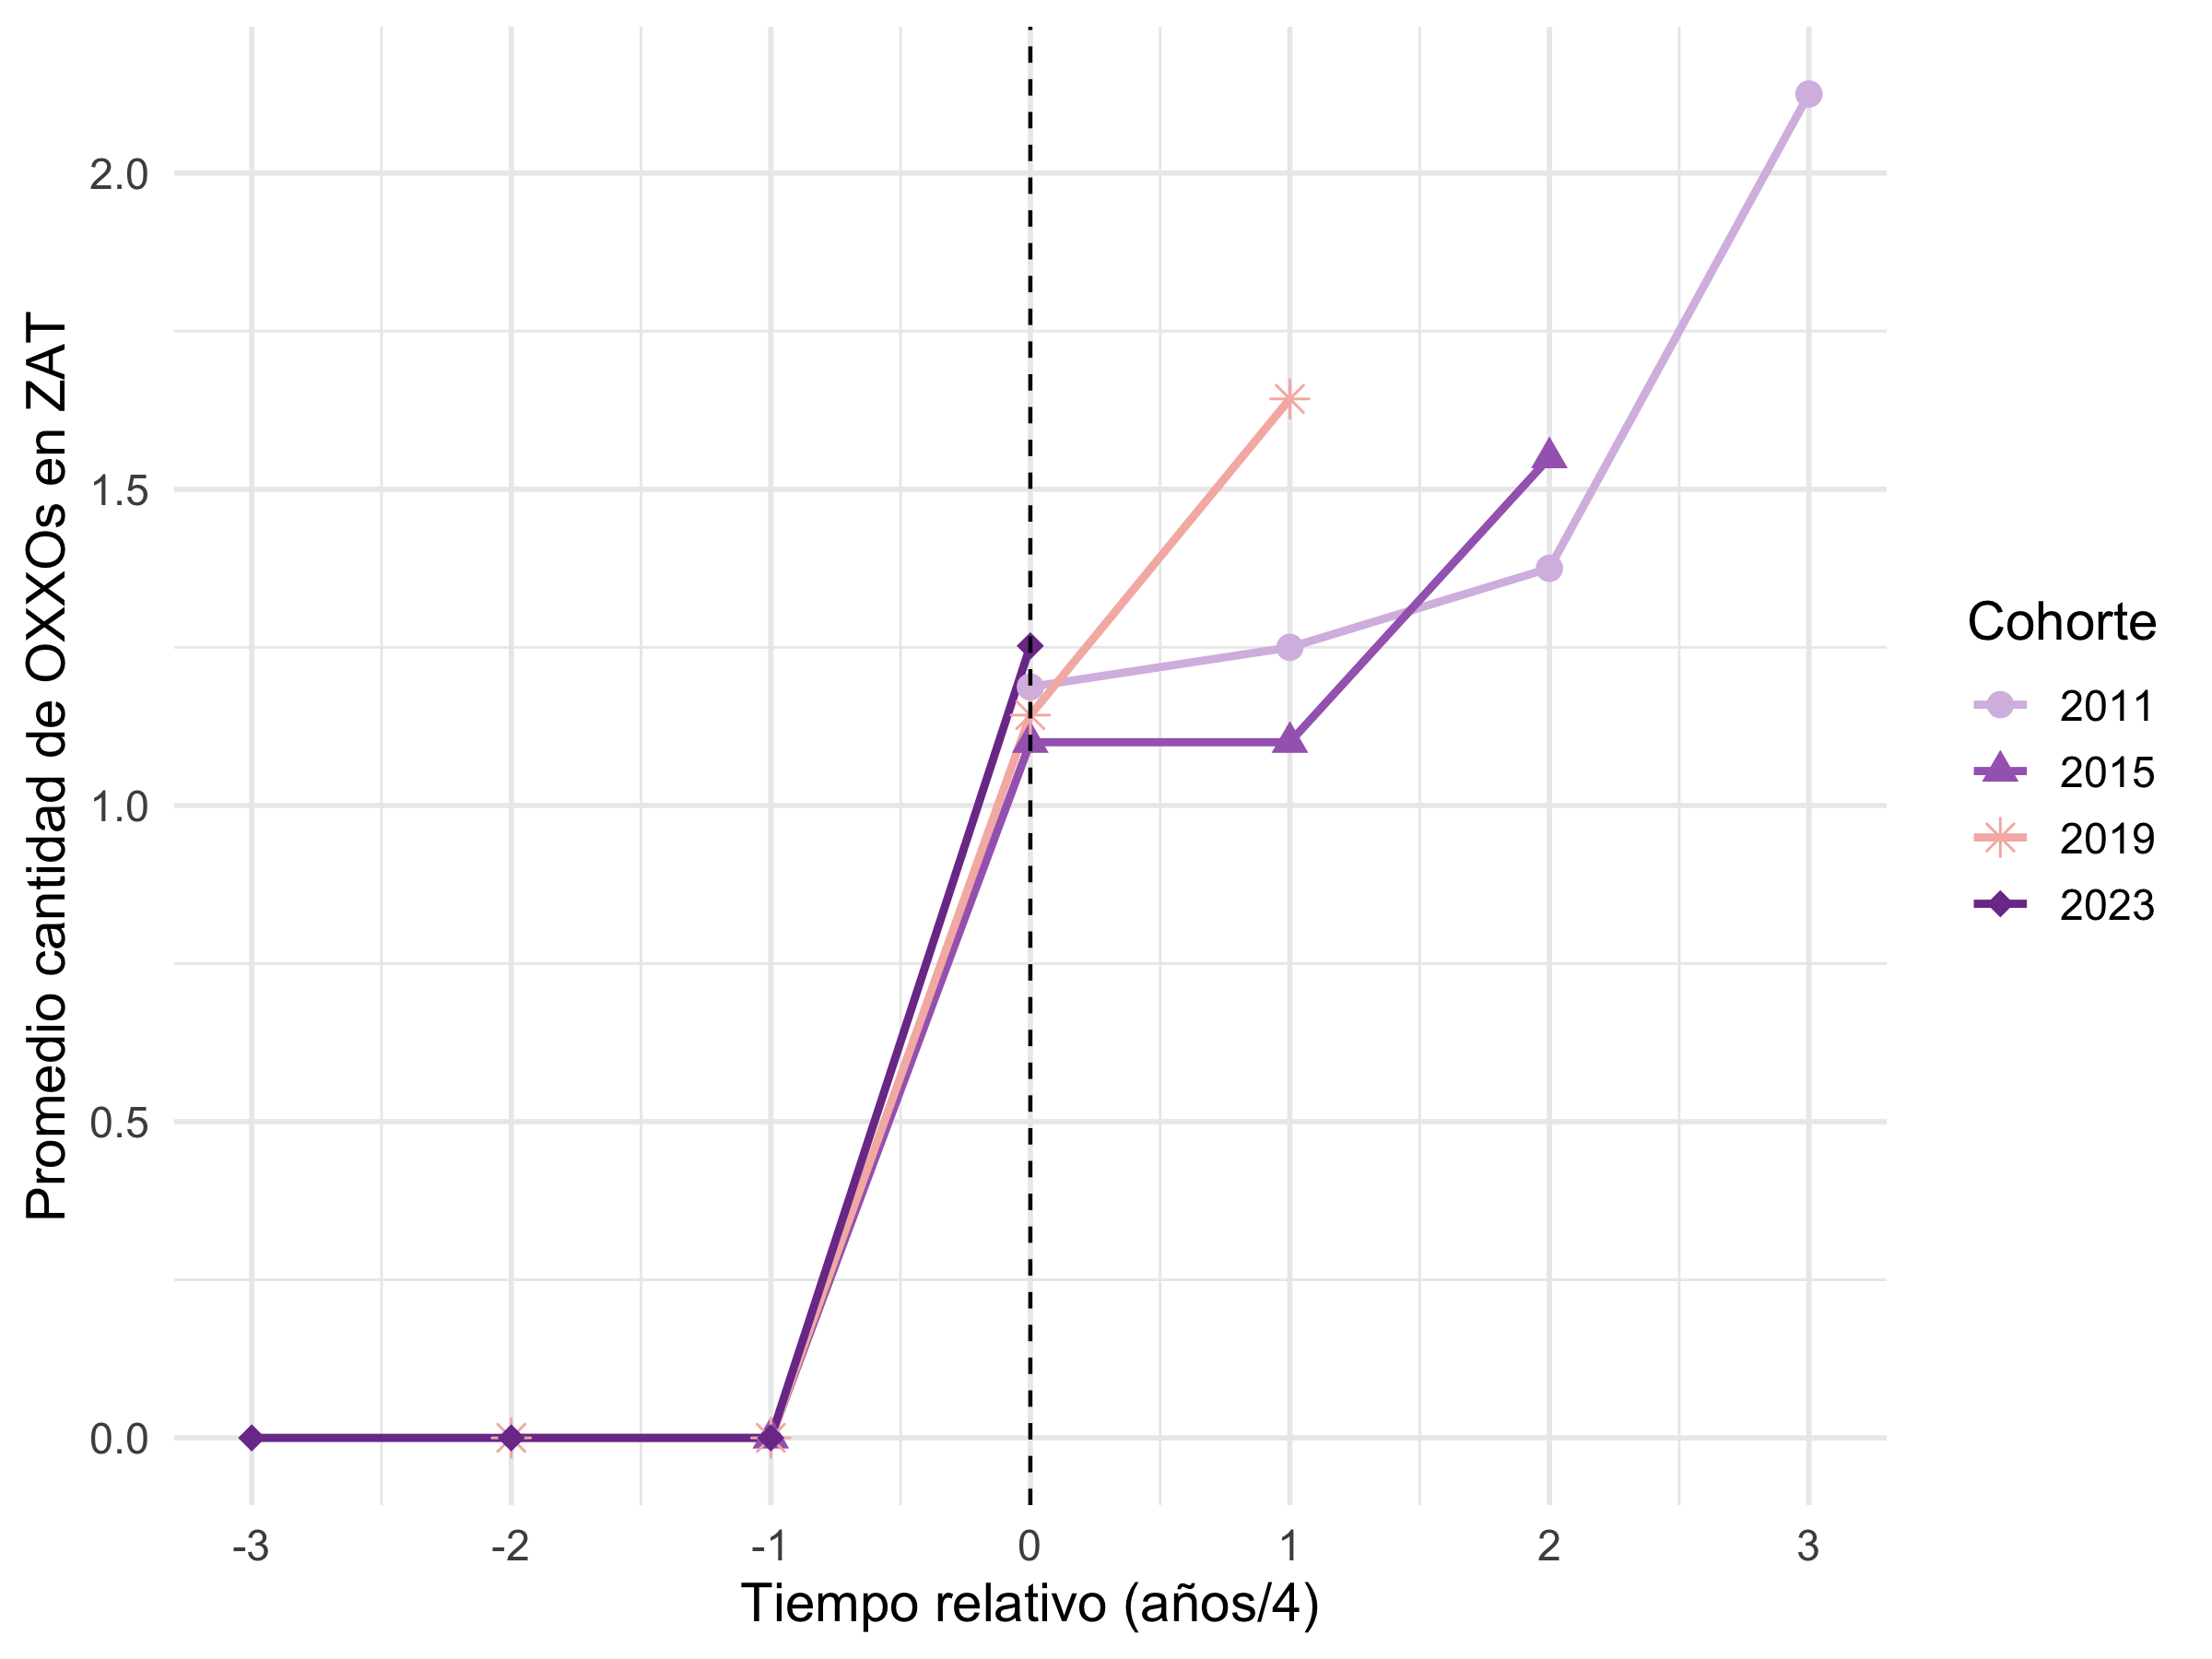
\includegraphics[width=0.6\linewidth]{other_figs/oxxos_intensidad_tratamiento.png} % Ajusta el path y tamaño
    \caption{
        \textbf{Evolución relativa promedio de cantidad de OXXOs por ZAT por cohorte} 
        \newline
        \footnotesize{\textit{Nota:} Esta figura muestra la evoluación promedio de la cantidad de OXXOs por ZAT para cada cohorte. El tiempo cero indica el año en que el cohorte inicia a ser tratado. Un rezago o adelanto representa una diferencia de 4 años. }
     }   
    \label{fig:intensidad}
\end{figure}

\begin{figure} [H]
    \centering
    % Top-left
    \begin{subfigure}[b]{0.4\textwidth} % Valor ajustado aquí
        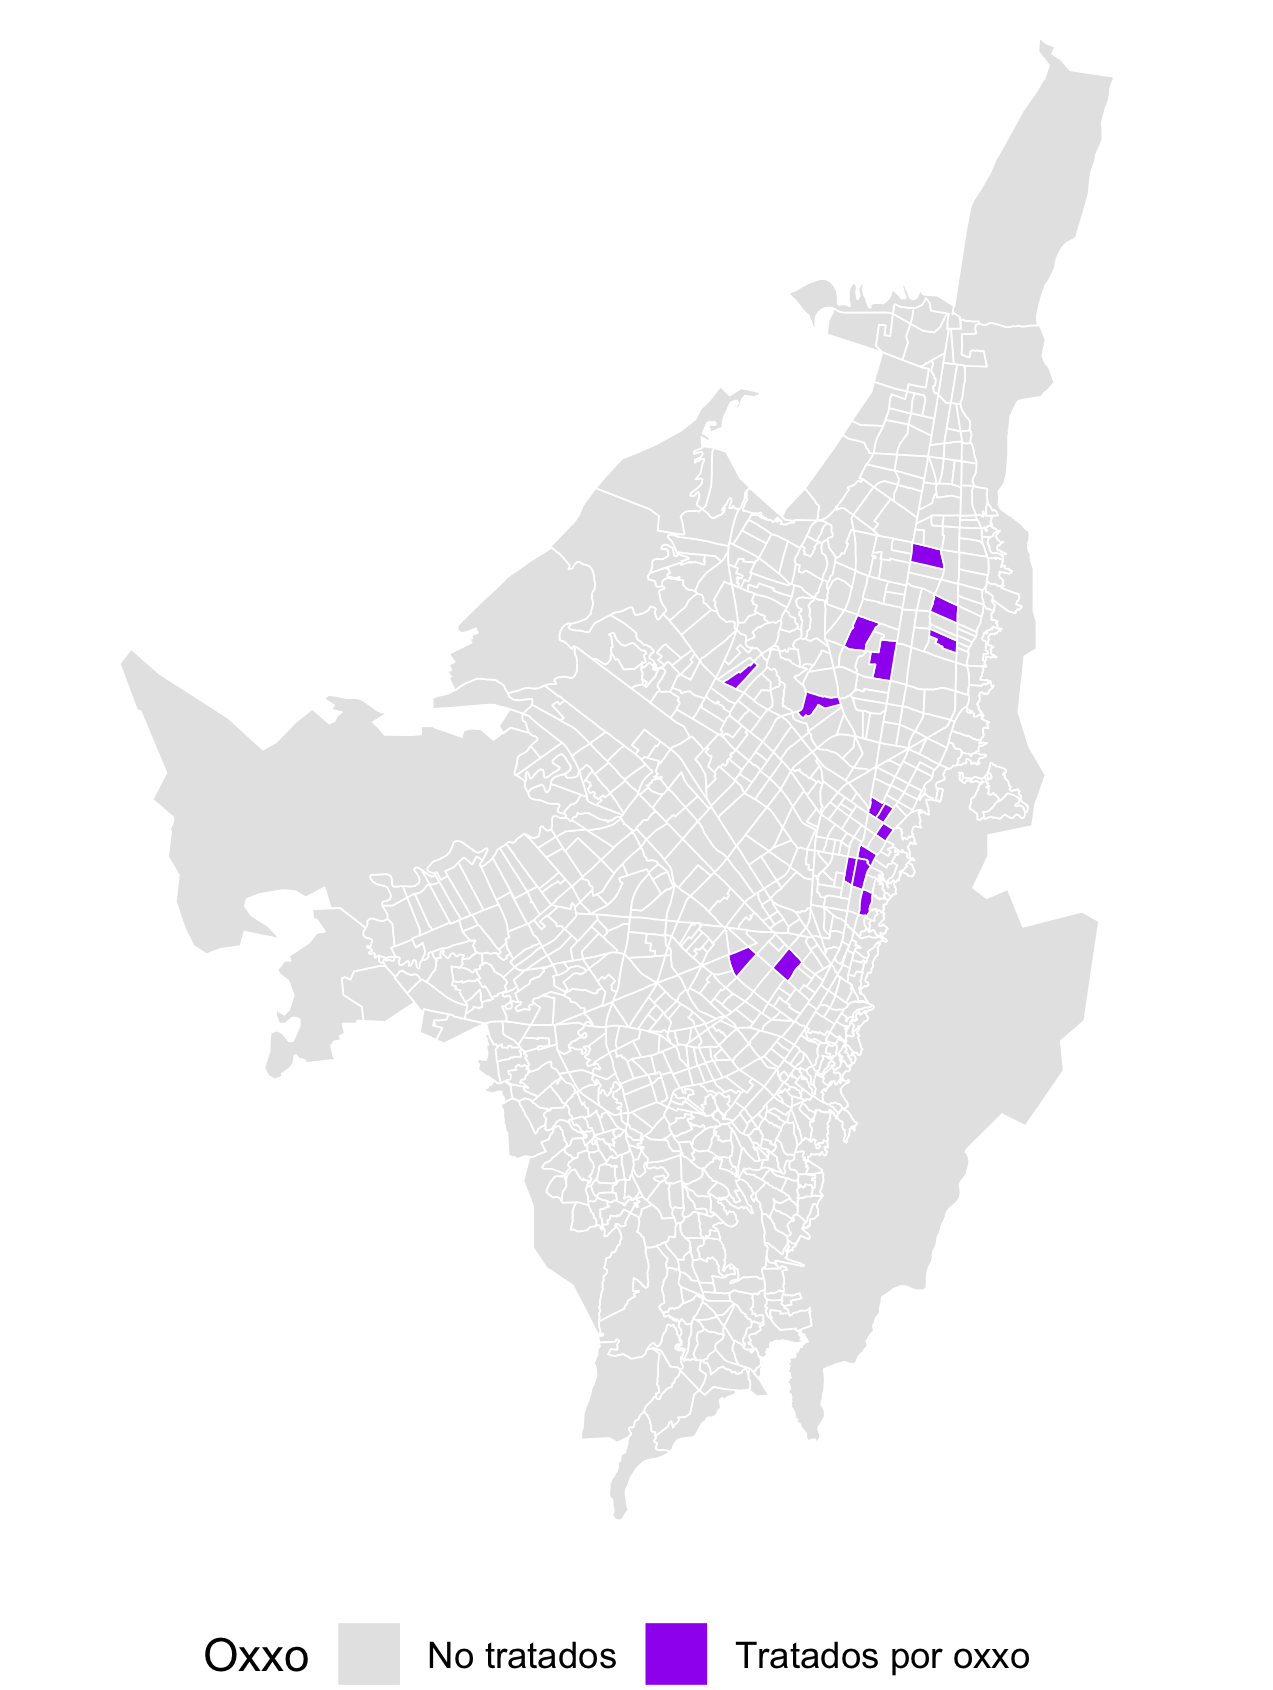
\includegraphics[width=\linewidth]{figs_oxxo_maps/mapa_oxxos_binary_2011.png}
        \caption{Panel A: OXXOs por ZAT en el 2011}
        \label{fig:panelA}
    \end{subfigure}
    \hfill
    % Top-right
    \begin{subfigure}[b]{0.4\textwidth} % Valor ajustado aquí
        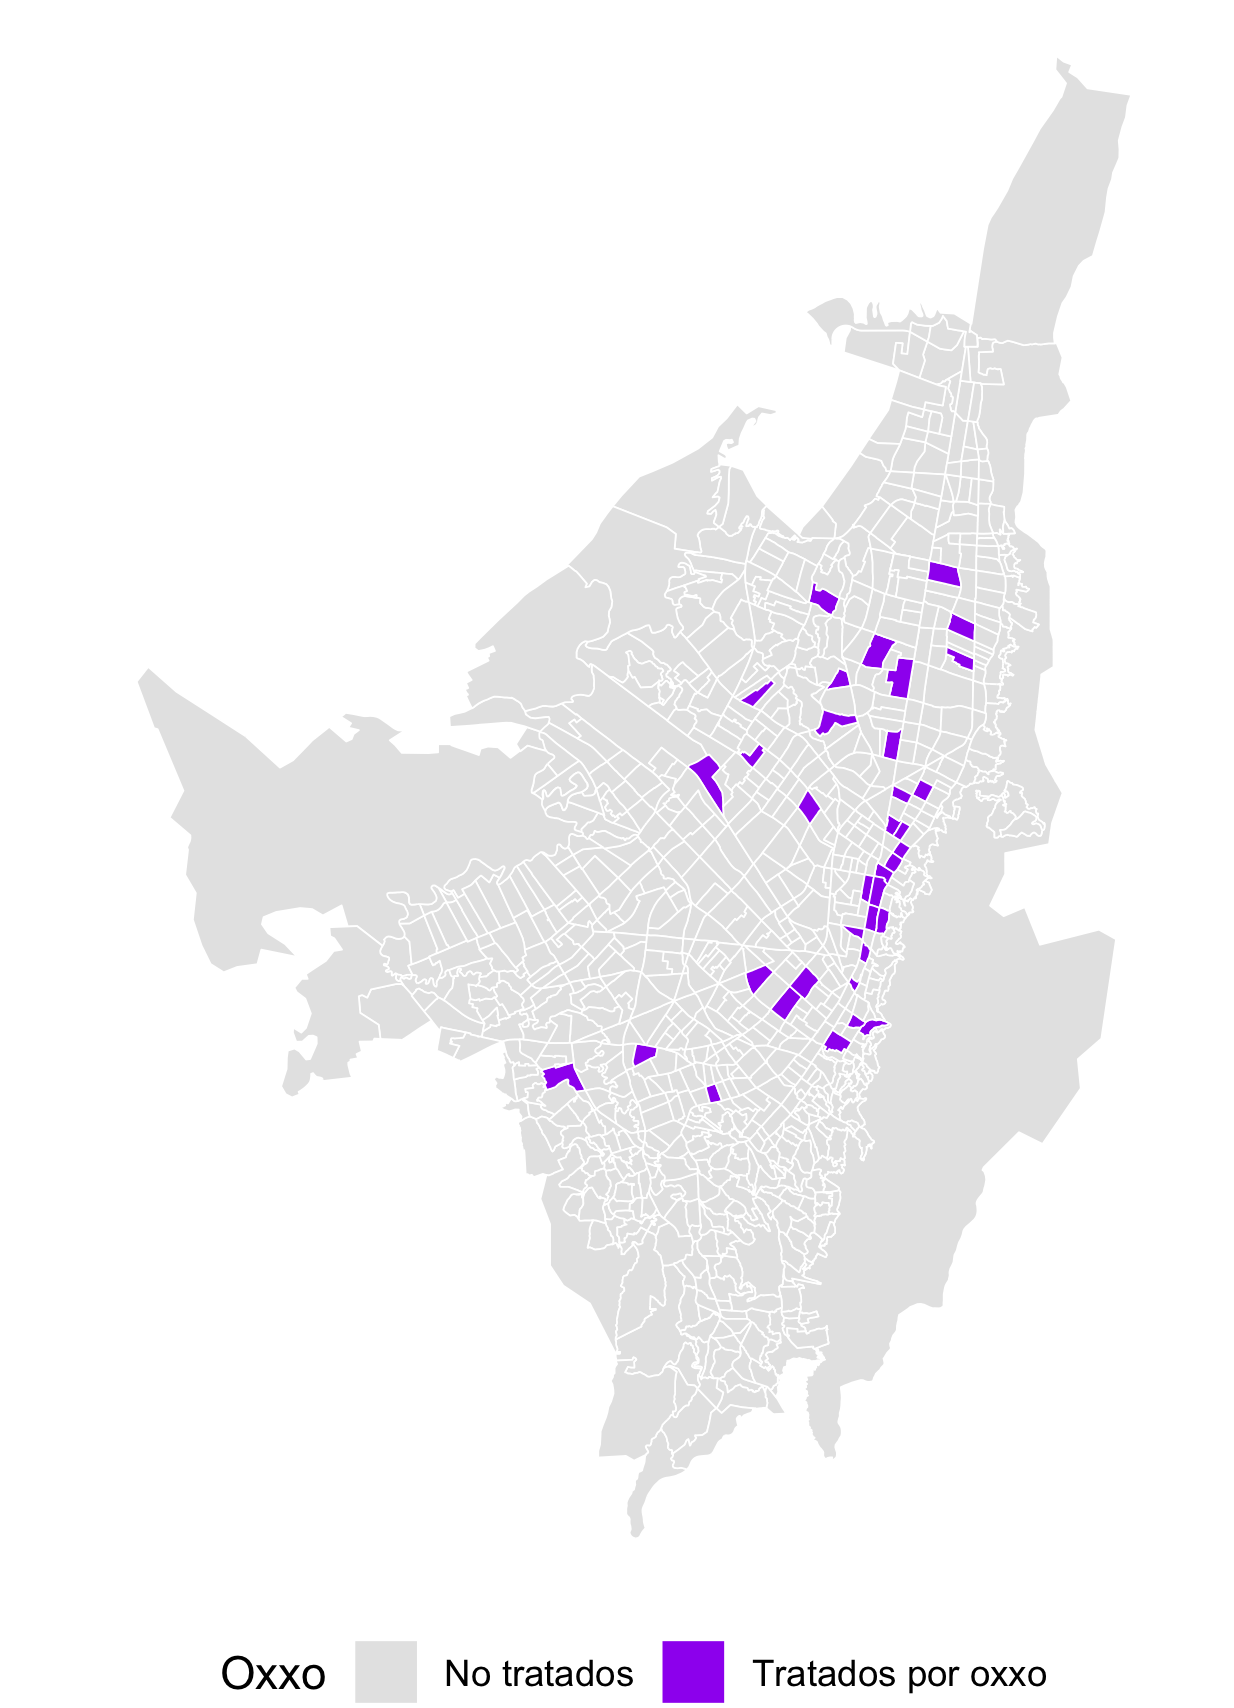
\includegraphics[width=\linewidth]{figs_oxxo_maps/mapa_oxxos_binary_2015.png}
        \caption{Panel B: OXXOs por ZAT en el 2015}
        \label{fig:panelB}
    \end{subfigure}
    
    \vspace{0.5cm}
    
    % Bottom-left
    \begin{subfigure}[b]{0.4\textwidth} % Valor ajustado aquí
        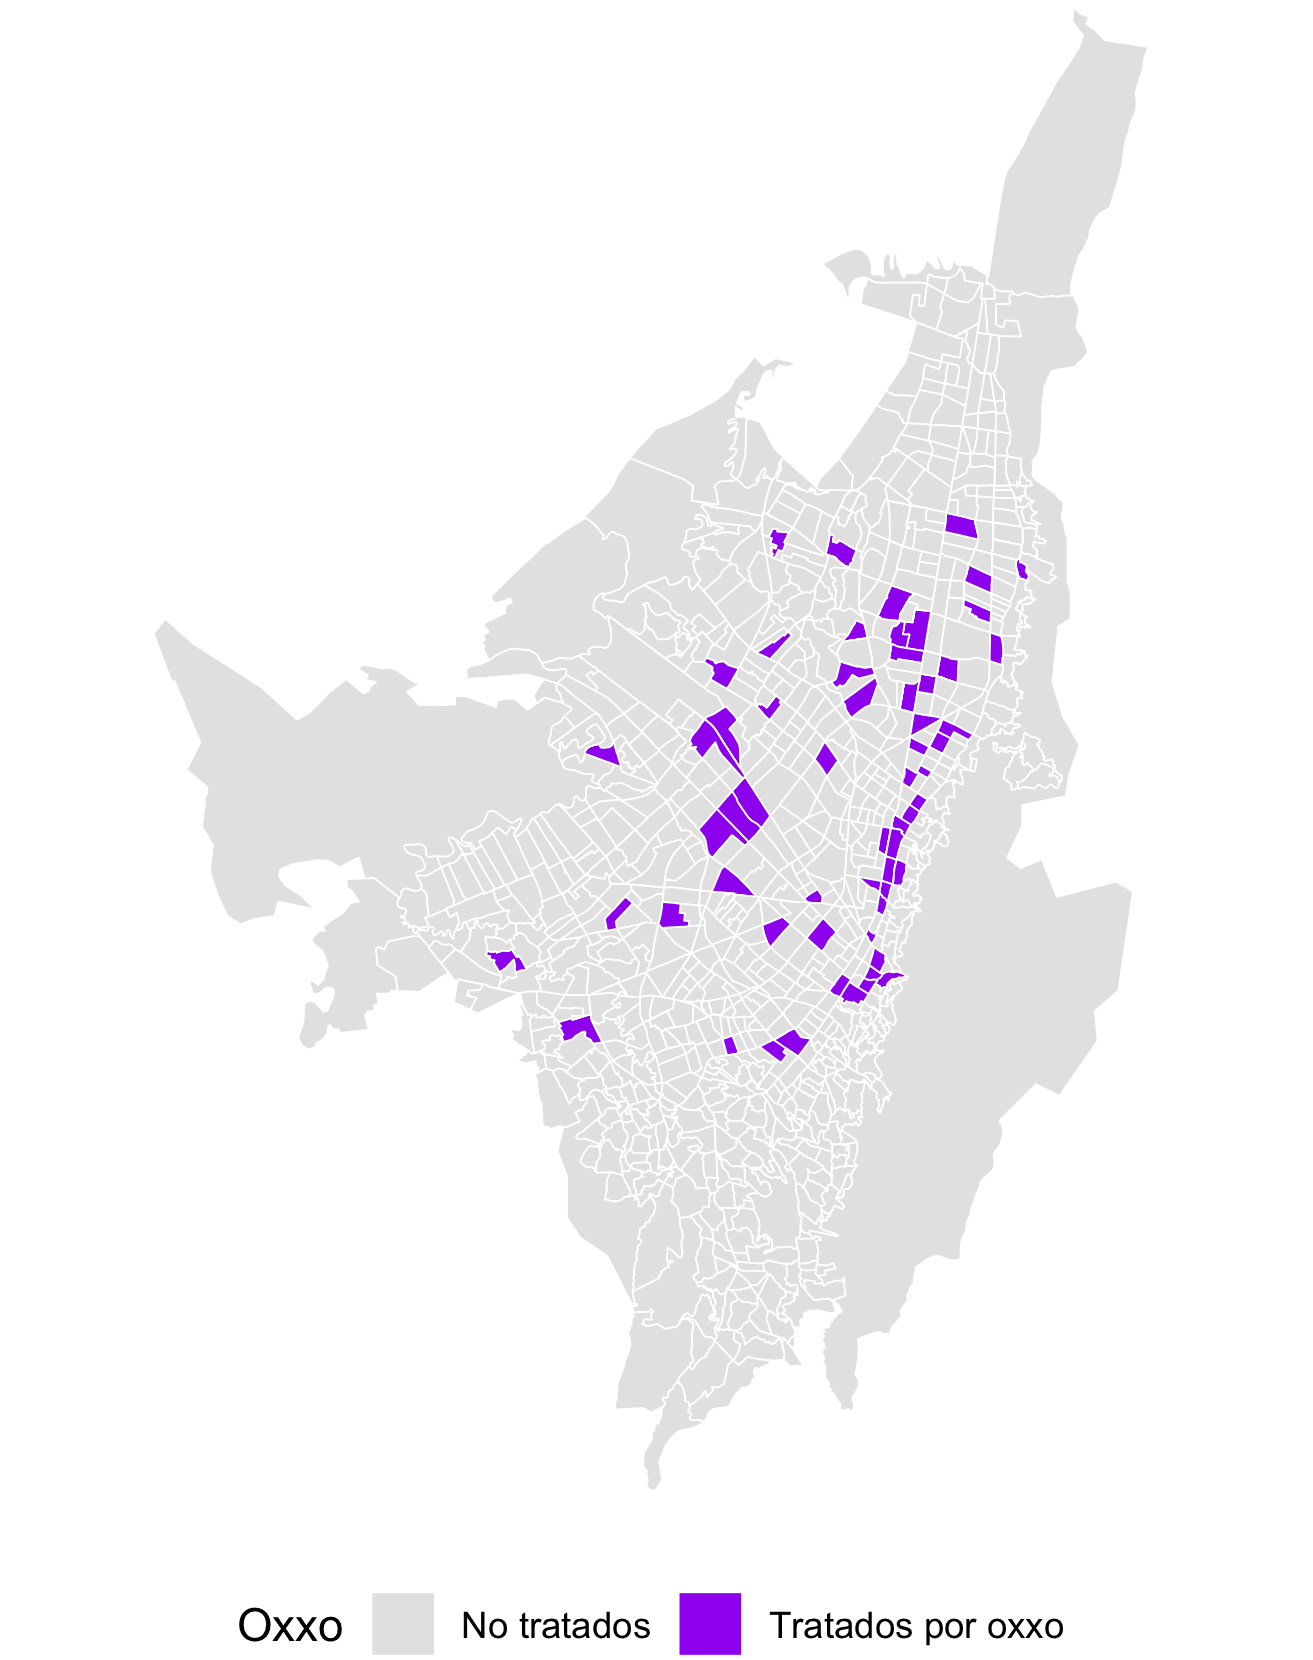
\includegraphics[width=\linewidth]{figs_oxxo_maps/mapa_oxxos_binary_2019.png}
        \caption{Panel C: OXXOs por ZAT en el 2019}
        \label{fig:panelC}
    \end{subfigure}
    \hfill
    % Bottom-right
    \begin{subfigure}[b]{0.4\textwidth} % Valor ajustado aquí
        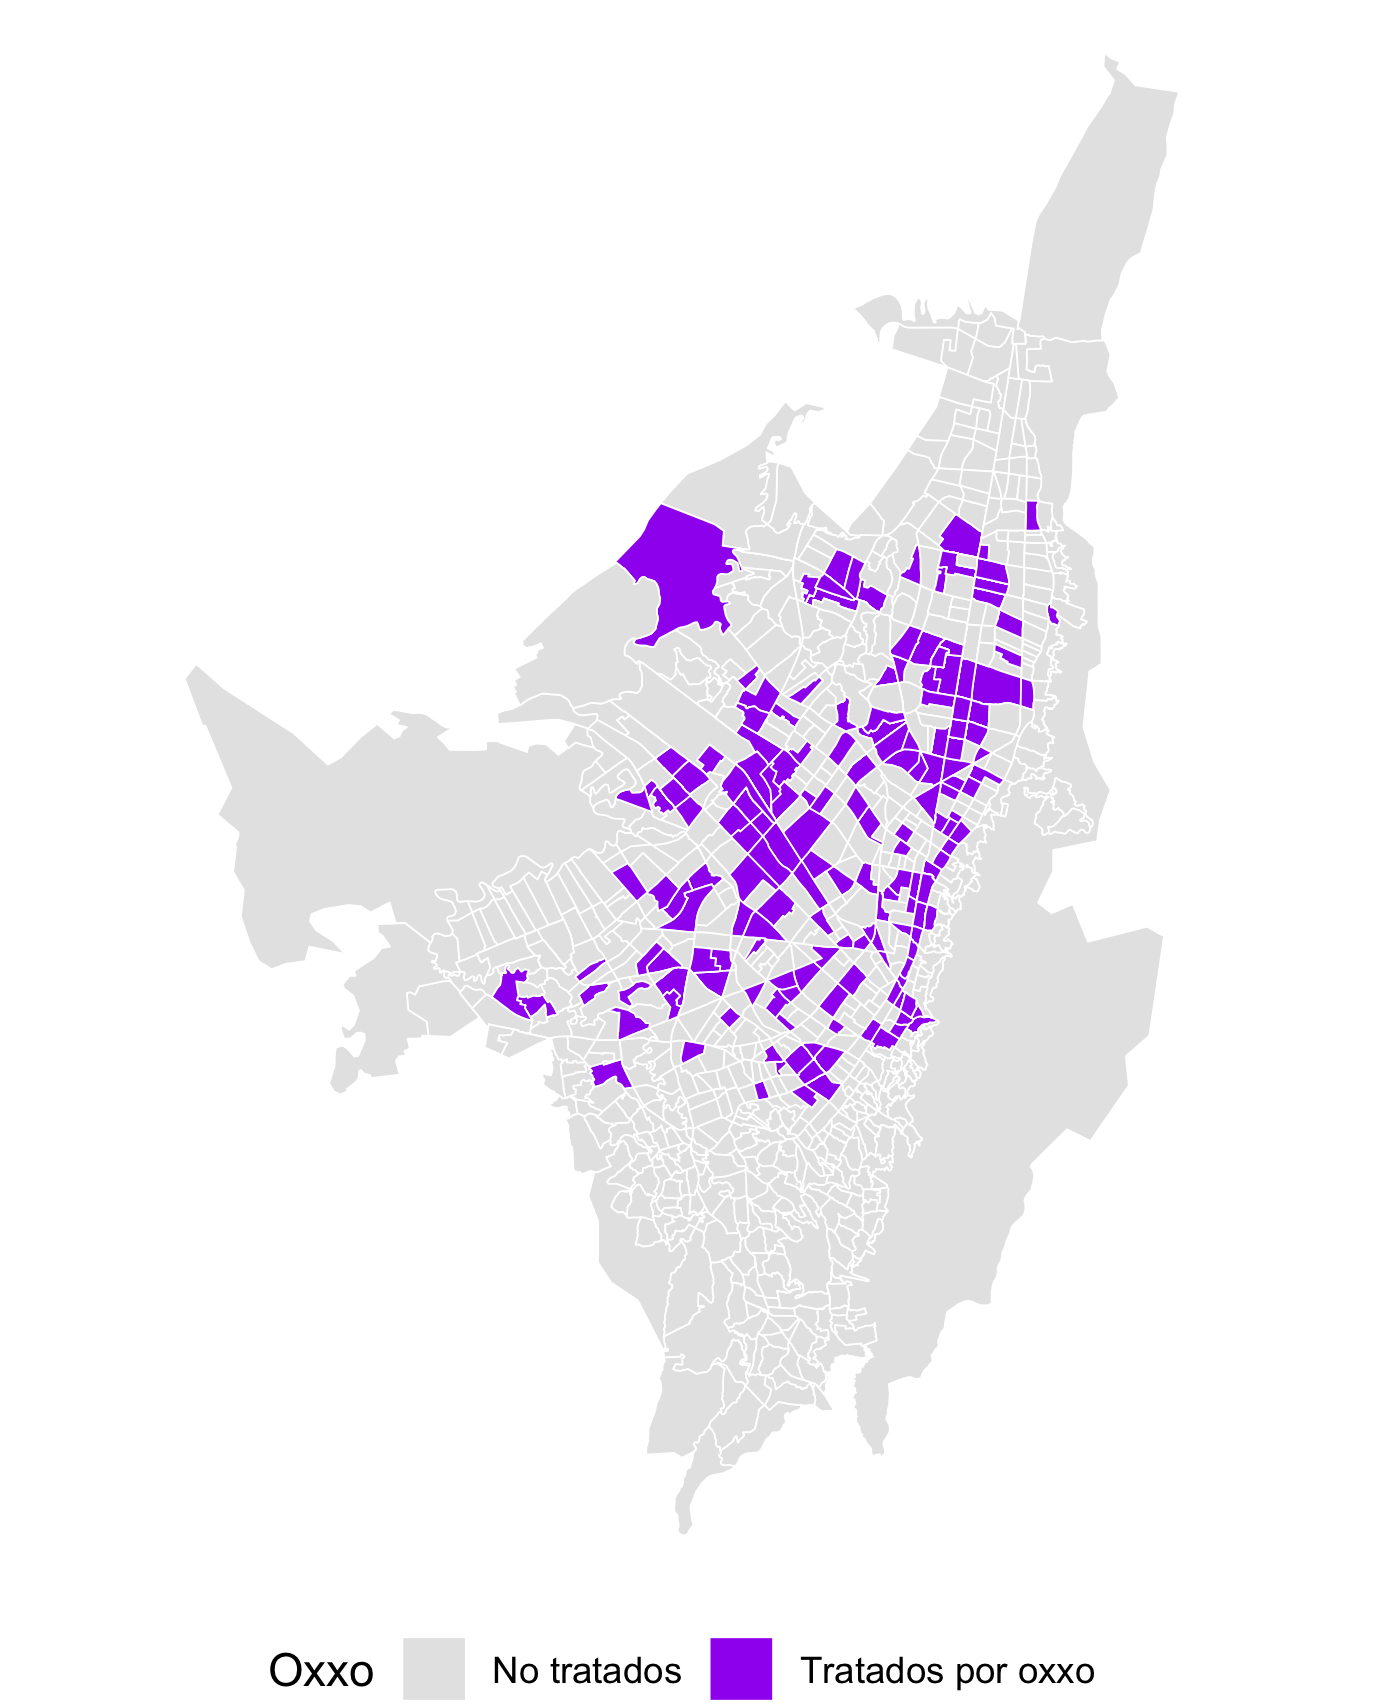
\includegraphics[width=\linewidth]{figs_oxxo_maps/mapa_oxxos_binary_2023.png}
        \caption{Panel D: OXXOs por ZAT en el 2023}
        \label{fig:panelD}
    \end{subfigure}
    
    \caption{
        \textbf{Evolución de la presencia de OXXOs por ZAT}
    }
    \label{fig:fourpanelOXXO}
\end{figure}


\section{Variables de control}

Los controles de línea base y fijos en el tiempo están en la Tabla~\ref{tab:diferencias_medias_controles_fijos}. Estos no serán necesarios ya que el TWFE inherentemente controla por caracteristicas constantes en unidad y tiempo. No obstante, ayudan a entender que los OXXO se ubican en zonas donde hay mayor tráfico, accesibilidad, poder adquisitivo y tamaño del mercado (reflejado por el tamaño del hogar). Esto va en línea con lo confirmado por \textcite{marcos2022} , donde las cadenas de conveniencia en México resultaron distrubirse por esas características.  Adicionalmente, los controles variables afirman los resultados de los fijos. Para cada cohorte, el ingreso y tamaño del hogar por ZAT resulta ser significativo (revisar apéndice~\ref{sec:controles_variables}). \\


\begin{table} [H]
  \centering
  \caption{Diferencias de medias entre tratados y nunca tratados para controes fijos}
  \label{tab:diferencias_medias_controles_fijos}
  \begin{adjustbox}{width=\textwidth,center}
    \begin{tabular}{l c c c}
      \toprule
      \multicolumn{1}{c}{} & \multicolumn{1}{c}{\textbf{Nunca tratados}} & \multicolumn{1}{c}{\textbf{Tratados}} & \multicolumn{1}{c}{\textbf{Diferencia de medias}} \\
      \midrule
       \midrule
      \multicolumn{4}{l}{\textbf{Línea base}} \\
      \midrule
      Habitantes por localidad en 2007 & 481.997 & 473.073 & -8.924 \\
      & (11.180) & (26.920) & \\
      Cantidad de personas por hogar 2007 & 3.522 & 3.298 & $-0.225^{***}$ \\
      & (0.015) & (0.030) & \\
      Indice de condiciones de vida 2007 & 89.121 & 91.724 & $2.603^{***}$ \\
      & (0.151) & (0.216) & \\
      Gasto promedio mensual 2007 & $1.02e+06$ & $1.28e+06$ & $2.54e+05^{***}$ \\
      & $(22613.352)$ & $(50141.458)$ & \\
      \midrule
      \multicolumn{4}{l}{\textbf{Controles fijos}} \\
      \midrule
      Estrato promedio & 2.722 & 3.483 & $0.761^{***}$ \\
      & (0.047) & (0.073) & \\
      Estaciones de transmilenio cercanas & 1.746 & 3.433 & $1.687^{***}$ \\
      & (0.088) & (0.221) & \\
      Cantidad acceso a vías arteriales & 3.830 & 6.234 & $2.404^{***}$ \\
      & (0.103) & (0.292) & \\
      \midrule
      \midrule
      ZATs & 725 & 171 & 896 \\
      \bottomrule
    \end{tabular}
  \end{adjustbox}
   \parbox[t]{\textwidth}{%
    \vspace{0.5em}
    \footnotesize{ \textit{Nota:} Significancia: *** p<0.01, ** p<0.05, * p<0.1.}}
\end{table}

Por su parte, los controles de las cadenas de D1 y ARA resultaron ser significativos (revisar apéndice~\ref{sec:controles_cadenas_descuento}). Esto resalta la importancia de su inclusión, porque indica que su presencia influye en el tratamiento; los minoristas suelen agruparse en ciertas áreas para aprovechar los beneficios de la aglomeración \parencite{Konishi2005, Seong2022}. Además, se conoce que la presencia de tiendas de descuento duro puede afectar la variable dependiente \parencite{delgado2024}. \\

Finalmente, se realizó una diferencia de medias entre los cortes transversales de las Encuestas de Movilidad. Se pudo observar que existían diferencias significativas que podían afectar a la variable dependiente. Por tanto, los cortes transversales repetidos no son comparables y es necesario incluir dichos controles (revisar apéndice~\ref{sec:controles_cortes_transversales}). \\

\newpage
\printbibliography

\newpage

\section{Apéndice}

\appendix
\counterwithin{table}{section}
\counterwithin{figure}{section}

\section{Controles línea base por cohortes}
\label{sec:controles_linea_base}

\begin{table} [H]
  \centering
  \caption{Diferencia de medias de controles de línea base para el cohorte 2011}
  \label{tab:comparacion_2011}
  \begin{tabular}{l c c c}
    \toprule
    & \textbf{Aún sin tratar} & \textbf{Tratados} & \textbf{Diferencia de medias} \\
    \midrule
    \multicolumn{4}{l}{\textbf{Línea base}} \\
    \midrule
    Habitantes por localidad en 2007 & 481.890 & 392.478 & -89.413 \\
    & (10.465) & (87.608) & \\
    cantidad de personas por hogar 2007 & 3.489 & 2.971 & $-0.518^{***}$ \\
    & (0.014) & (0.116) & \\
    Indice de condiciones de vida 2007 & 89.539 & 93.955 & $4.416^{***}$ \\
    & (0.134) & (0.640) & \\
    gasto promedio mensual 2007 & $1.06e+06$ & $1.79e+06$ & $7.35e+05^{***}$ \\
    & (20917.105) & (1.21e+05) & \\
    \midrule
    \multicolumn{4}{l}{\textbf{Controles fijos}} \\
    \midrule
    estrato promedio & 2.864 & 3.801 & $0.937^{***}$ \\
    & (0.042) & (0.193) & \\
    Estaciones de transmilenio cercanas & 2.039 & 3.688 & $1.649^{**}$ \\
    & (0.087) & (0.454) & \\
    Cantidad acceso a vías arteriales & 4.223 & 7.938 & $3.715^{***}$ \\
    & (0.103) & (0.292) & \\
    \midrule
    \textbf{ZATs} & 880 & 16 & 896 \\
    \bottomrule
  \end{tabular}
  \parbox[t]{\textwidth}{%
    \vspace{0.5em}
    \footnotesize{ \textit{Nota:} Significancia: *** p<0.01, ** p<0.05, * p<0.1.}}
\end{table}

\begin{table} [H]
  \centering
  \caption{Diferencia de medias de controles de línea base para el cohorte 2015}
  \label{tab:comparacion_2015}
  \begin{tabular}{l c c c}
    \toprule
    & \textbf{Aún sin tratar} & \textbf{Tratados} & \textbf{Diferencia de medias} \\
    \midrule
    \multicolumn{4}{l}{\textbf{Línea base}} \\
    \midrule
    Habitantes por localidad en 2007 & 484.916 & 369.880 & -115.035$^{**}$ \\
    & (10.529) & (58.628) & \\
    cantidad de personas por hogar 2007 & 3.497 & 3.075 & $-0.422^{***}$ \\
    & (0.014) & (0.079) & \\
    Indice de condiciones de vida 2007 & 89.501 & 92.409 & $2.908^{***}$ \\
    & (0.136) & (0.591) & \\
    gasto promedio mensual 2007 & $1.06e+06$ & $1.47e+06$ & $4.15e+05^{***}$ \\
    & (21062.412) & (1.15e+05) & \\
    \midrule
    \multicolumn{4}{l}{\textbf{Controles fijos}} \\
    \midrule
    estrato promedio & 2.842 & 3.735 & $0.893^{***}$ \\
    & (0.042) & (0.161) & \\
    Estaciones de transmilenio cercanas & 1.984 & 4.083 & $2.100^{**}$ \\
    & (0.087) & (0.422) & \\
    Cantidad acceso a vías arteriales & 4.176 & 7.000 & $2.824^{***}$ \\
    & (0.103) & (0.715) & \\
    \midrule
    \textbf{ZATs} & 860 & 36 & 896 \\
    \bottomrule
  \end{tabular}
  \parbox[t]{\textwidth}{%
    \vspace{0.5em}
    \footnotesize{ \textit{Nota:} Significancia: *** p<0.01, ** p<0.05, * p<0.1.}}
\end{table}

\begin{table} [H]
  \centering
  \caption{Diferencia de medias de controles de línea base para el cohorte 2019}
  \label{tab:comparacion_2019}
  \begin{tabular}{l c c c}
    \toprule
    & \textbf{Aún sin tratar} & \textbf{Tratados} & \textbf{Diferencia de medias} \\
    \midrule
    \multicolumn{4}{l}{\textbf{Línea base}} \\
    \midrule
    Habitantes por localidad en 2007 & 485.354 & 411.027 & -74.327$^{*}$ \\
    & (10.662) & (44.380) & \\
    cantidad de personas por hogar 2007 & 3.503 & 3.153 & $-0.350^{***}$ \\
    & (0.014) & (0.059) & \\
    Indice de condiciones de vida 2007 & 89.440 & 92.409 & $2.615^{***}$ \\
    & (0.138) & (0.424) & \\
    gasto promedio mensual 2007 & $1.05e+06$ & $1.41e+06$ & $3.60e+05^{***}$ \\
    & (21241.687) & (88739.694) & \\
    \midrule
    \multicolumn{4}{l}{\textbf{Controles fijos}} \\
    \midrule
    estrato promedio & 2.818 & 3.671 & $0.853^{***}$ \\
    & (0.043) & (0.141) & \\
    Estaciones de transmilenio cercanas & 1.941 & 3.803 & $1.862^{**}$ \\
    & (0.087) & (0.352) & \\
    Cantidad acceso a vías arteriales & 4.111 & 6.721 & $2.610^{***}$ \\
    & (0.102) & (0.550) & \\
    \midrule
    \textbf{ZATs} & 896 & 61 & 896 \\
    \bottomrule
  \end{tabular}
  \parbox[t]{\textwidth}{%
    \vspace{0.5em}
    \footnotesize{ \textit{Nota:} Significancia: *** p<0.01, ** p<0.05, * p<0.1.}}
\end{table}

\begin{table} [H]
  \centering
  \caption{2023 - entre tratados y nunca tratados}
  \label{tab:comparacion_tratamientos}
  \begin{tabular}{l c c c}
    \toprule
    & \textbf{Aún sin tratar} & \textbf{Tratados} & \textbf{Diferencia de medias} \\
    \midrule
    \multicolumn{4}{l}{\textbf{Línea base}} \\
    \midrule
    Habitantes por localidad en 2007 & 481.997 & 473.073 & -8.924 \\
    & (11.180) & (26.920) & \\
    cantidad de personas por hogar 2007 & 3.522 & 3.298 & $-0.225^{***}$ \\
    & (0.015) & (0.030) & \\
    Indice de condiciones de vida 2007 & 89.121 & 91.724 & $2.603^{***}$ \\
    & (0.151) & (0.216) & \\
    gasto promedio mensual 2007 & $1.02e+06$ & $1.28e+06$ & $2.54e+05^{***}$ \\
    & (22613.352) & (50141.458) & \\
    \midrule
    \multicolumn{4}{l}{\textbf{Controles fijos}} \\
    \midrule
    estrato promedio & 2.722 & 3.483 & $0.761^{***}$ \\
    & (0.047) & (0.073) & \\
     Estaciones de transmilenio cercanas & 1.746 & 3.433 & $1.687^{***}$ \\
    & (0.088) & (0.221) & \\
    Cantidad acceso a vías arteriales & 3.830 & 6.234 & $2.404^{***}$ \\
    & (0.103) & (0.292) & \\
    \midrule
    \midrule
    \textbf{ZATs} & 725 & 171 & 896 \\
    \bottomrule
  \end{tabular}
  \parbox[t]{\textwidth}{%
    \vspace{0.5em}
    \footnotesize{ \textit{Nota:} Significancia: *** p<0.01, ** p<0.05, * p<0.1.}}
\end{table}

\section{Controles rezagados de cadenas de descuento por cohorte}
\label{sec:controles_cadenas_descuento}

Los resultados de las diferencas de medias de cadenas de descuento duro por cohorte muestra resultados significativos dependiendo del cohorte.\\

No se incluyó una tabla para el 2011, porque ni los D1s, ni los J\&Bs, ni los ARAs habian llegado a Bogotá. Para el 2015 únicamente había tiendas D1, por lo que solo se evaluó la diferencia para dicha cadena. \\

En 2019 los J\&B y ARA aparecen en el radar. En este año se puede observar que los J\&B no presentan diferencias significativas, por lo que no es un control necesario. Además, esto se afirma al observar que en 2023 J\&B ya había cerrado en el país. Por tanto, los unicos controles relevantes son D1 y ARA.\\

\begin{table} [H]
  \centering
  \caption{Diferencia de medias de controles de tiendas de descuento para el cohorte 2015}
  \label{tab:d1}
  \begin{tabular}{l c c c}
    \toprule
    & \textbf{Aún sin tratar} & \textbf{Tratados} & \textbf{Diferencia de medias} \\
    \midrule
    Tiene D1 & 0.050 & 0.222 & $0.172^{***}$ \\
    & (0.007) & (0.070) & \\
    \midrule
    Cantidad de D1s & 0.062 & 0.278 & $0.216^{***}$ \\
    & (0.010) & (0.094) & \\
    \midrule
    ZATs & 860 & 36 & 896 \\
    \bottomrule
  \end{tabular}
  \parbox[t]{\textwidth}{%
    \vspace{0.5em}
    \footnotesize{ \textit{Nota:} Significancia: *** p<0.01, ** p<0.05, * p<0.1.}}
\end{table}

\begin{table} [H]
  \centering
  \caption{TDiferencia de medias de controles de tiendas de descuento para el cohorte 2019}
  \label{tab:d1_jb_ara}
  \begin{tabular}{l c c c}
    \toprule
    & \textbf{Aún sin tratar} & \textbf{Tratados} & \textbf{Diferencia de medias} \\
    \midrule
    Tiene J\&B & 0.083 & 0.098 & 0.016 \\
    & (0.010) & (0.038) & \\
    Tiene D1 & 0.170 & 0.410 & $0.240^{***}$ \\
    & (0.013) & (0.063) & \\
    Tiene ARA & 0.081 & 0.148 & $0.066^{*}$ \\
    & (0.009) & (0.046) & \\
    Cantidad de J\&B & 0.168 & 0.230 & 0.062 \\
    & (0.033) & (0.120) & \\
    Cantidad de D1s & 0.229 & 0.557 & $0.329^{***}$ \\
    & (0.022) & (0.098) & \\
    Cantidad de ARAs & 0.103 & 0.197 & $0.094^{*}$ \\
    & (0.013) & (0.069) & \\
    \midrule
    ZATs & 835 & 61 & 896 \\
    \bottomrule
  \end{tabular}
  \parbox[t]{\textwidth}{%
    \vspace{0.5em}
    \footnotesize{ \textit{Nota:} Significancia: *** p<0.01, ** p<0.05, * p<0.1.}}
\end{table}

\begin{table} [H]
  \centering
  \caption{Diferencia de medias de controles de tiendas de descuento para el cohorte 2023}
  \label{tab:d1_ara_2023}
  \begin{tabular}{l c c c}
    \toprule
    & \textbf{Aún sin tratar} & \textbf{Tratados} & \textbf{Diferencia de medias} \\
    \midrule
    Tiene D1 & 0.214 & 0.456 & $0.242^{***}$ \\
    & (0.015) & (0.038) & \\
    Tiene ARA & 0.109 & 0.246 & $0.137^{***}$ \\
    & (0.012) & (0.033) & \\
    Cantidad de D1s & 0.288 & 0.865 & $0.577^{***}$ \\
    & (0.025) & (0.118) & \\
    Cantidad de ARAs & 0.143 & 0.357 & $0.213^{***}$ \\
    & (0.017) & (0.056) & \\
    \midrule
    ZATs & 725 & 171 & 896 \\
    \bottomrule
  \end{tabular}
  \parbox[t]{\textwidth}{%
    \vspace{0.5em}
    \footnotesize{ \textit{Nota:} Significancia: *** p<0.01, ** p<0.05, * p<0.1.}}
\end{table}

\section{Controles variables por cohorte}
\label{sec:controles_variables}

% ---------------- 2011 ----------------
\begin{table} [H]
  \centering
  \caption{Diferencia de medias de controles de variables para el cohorte 2011}
  \label{tab:balance_2011}
  \begin{tabular}{l c c c}
    \toprule
    & \textbf{Aún sin tratar} & \textbf{Tratados} & \textbf{Diferencia de medias} \\
    \midrule
    Total personas & 3.526 & 4.016 & $0.490$ \\
    & (0.059) & (0.097) & \\
    Ingreso & 2.277 & 3.102 & $0.825^{**}$ \\
    & (0.044) & (0.103) & \\
    \midrule
    ZATs & 880 & 16 & 896 \\
    \bottomrule
  \end{tabular}
  \vspace{0.2cm}
  
\parbox[t]{\textwidth}{%
    \vspace{0.5em}
    \footnotesize{ \textit{Nota:} Significancia: *** p<0.01, ** p<0.05, * p<0.1.}}
  
\end{table}

% ---------------- 2015 ----------------
\begin{table} [H]
  \centering
  \caption{Diferencia de medias de controles de variables para el cohorte 2015}
  \label{tab:balance_2015}
  \begin{tabular}{l c c c}
    \toprule
    & \textbf{Aún sin tratar} & \textbf{Tratados} & \textbf{Diferencia de medias} \\
    \midrule
    Total personas & 3.177 & 3.625 & $0.448^{*}$ \\
    & (0.047) & (0.041) & \\
    Ingreso & 2.088 & 2.830 & $0.742^{***}$ \\
    & (0.044) & (0.086) & \\
    \midrule
    ZATs & 860 & 36 & 896 \\
    \bottomrule
  \end{tabular}
  
\parbox[t]{\textwidth}{%
    \vspace{0.5em}
    \footnotesize{ \textit{Nota:} Significancia: *** p<0.01, ** p<0.05, * p<0.1.}}
  
\end{table}

% ---------------- 2019 ----------------
\begin{table} [H]
  \centering
  \caption{Diferencia de medias de controles de variables para el cohorte 2019}
  \label{tab:balance_2019}
  \begin{tabular}{l c c c}
    \toprule
    & \textbf{Aún sin tratar} & \textbf{Tratados} & \textbf{Diferencia de medias} \\
    \midrule
    Total personas & 3.314 & 3.585 & $0.271$ \\
    & (0.048) & (0.041) & \\
    Ingreso & 2.792 & 3.660 & $0.868^{***}$ \\
    & (0.052) & (0.092) & \\
    \midrule
    ZATs & 835 & 61 & 896 \\
    \bottomrule
  \end{tabular}
\parbox[t]{\textwidth}{%
    \vspace{0.5em}
    \footnotesize{ \textit{Nota:} Significancia: *** p<0.01, ** p<0.05, * p<0.1.}}
  \end{table}

% ---------------- 2023 ----------------
\begin{table} [H]
  \centering
  \caption{Diferencia de medias de controles de variables para el cohorte 2023}
  \label{tab:balance_2023}
  \begin{tabular}{l c c c}
    \toprule
    & \textbf{Aún sin tratar} & \textbf{Tratados} & \textbf{Diferencia de medias} \\
    \midrule
    Total personas & 3.193 & 3.449 & $0.256^{**}$ \\
    & (0.049) & (0.030) & \\
    Ingreso & 3.875 & 4.799 & $0.924^{***}$ \\
    & (0.067) & (0.068) & \\
    \midrule
    ZATs & 725 & 171 & 896 \\
    \bottomrule
  \end{tabular}
  \parbox[t]{\textwidth}{%
    \vspace{0.5em}
    \footnotesize{ \textit{Nota:} Significancia: *** p<0.01, ** p<0.05, * p<0.1.}}
  \vspace{0.2cm}
  \end{table}

\section{Controles por diferencias entre cortes transversales}
\label{sec:controles_cortes_transversales}


\end{document}
